\begin{statement}{5}
  For each case, compute the polynomial interpolant using $n$ second-kind
  Chebyshev nodes in $[-1, 1]$ for $n = 4, 8, 12, \dots, 60$.
  At each value of $n$, compute the infinity-norm error
  (that is, $\max|p(x) - f(x)|$ evaluated for at least $4000$ values of $x$).
  Using a log-linear scale, plot the error as a function of $n$,
  then determine a good approximation to the constant $k$ in
  \[
    \max_{x \in [-1, 1]} |f(x) - p(x)| \leq c k ^{-n},
  \]
  where $f$ is analytic in an open real interval containing $[-1, 1]$, $c > 0$ and $k > 1$.
\end{statement}

\begin{statement}{a}
  $f(x) = 1 / (25 x^2 + 1)$.
\end{statement}

\begin{solution}
  Computing the infinity-norm error of $4001$ evenly spaced points between $-1$ and $1$
  of each polynomial interpolant, a good approximation for $k$ is $1.85$ using $c = 1$.
  \lstinputlisting{scripts/problems/problem-05-01.m}
  \begin{figure}[H]
    \centering
    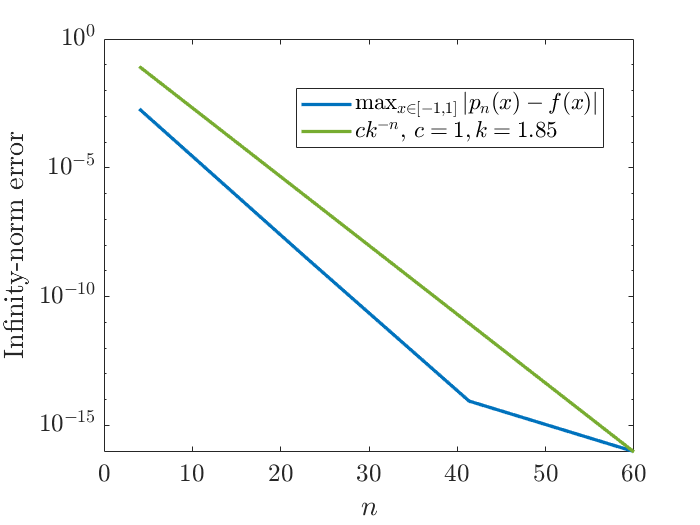
\includegraphics[scale=0.5]{graphics/plot-05-01.png}
    \caption{Infinity norm error of $f(x) = 1 / (25 x^2 + 1)$ and a bounding function}
  \end{figure}
\end{solution}

\begin{statement}{c}
  $f(x) = \cosh(\sin x)$.
\end{statement}

\begin{solution}
  Computing the infinity-norm error of $4001$ evenly spaced points between $-1$ and $1$
  of each polynomial interpolant, a good approximation for $k$ is $1.75$ using $c = 1$.
  \lstinputlisting{scripts/problems/problem-05-03.m}
  \begin{figure}[H]
    \centering
    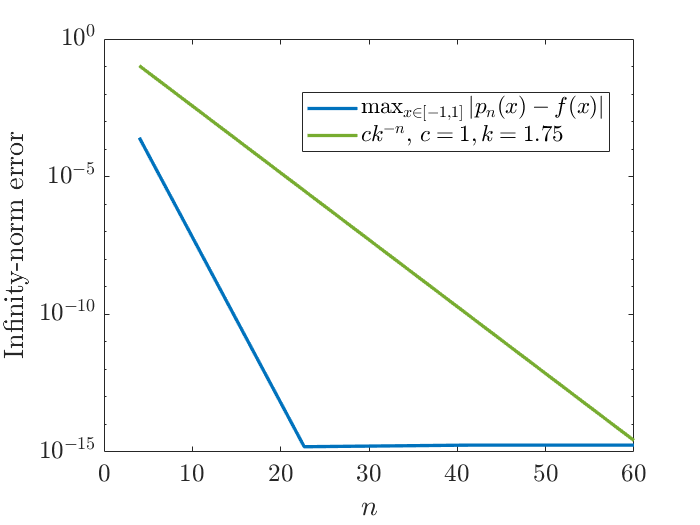
\includegraphics[scale=0.5]{graphics/plot-05-03.png}
    \caption{Infinite norm error of $f(x) = \cosh(\sin(x))$ and a bounding function}
  \end{figure}
\end{solution}